\documentclass[14pt]{beamer}


\mode<presentation>{
  \usetheme{Warsaw}

  \definecolor{beamer@blendedred}{rgb}{0.7,0.1,0.1}
  \setbeamercolor{structure}{fg=beamer@blendedred}

  \setbeamercovered{invisible}
}

\usepackage[T2A]{fontenc}
\usepackage[utf8]{inputenc}
\usepackage[russian]{babel}
\usepackage{multimedia}
\usepackage{hyperref}
\usepackage{setspace}
\linespread{1.3}
\logo{
\includegraphics[height=0.3cm]{valknut.png}}

%% \renewcommand{\rmdefault}{phv} % Arial
%% \renewcommand{\sfdefault}{phv} % Arial

\definecolor{ExclamMark}{RGB}{34, 89, 150}
\definecolor{darkgreen}{rgb}{0,0.5,0}
\definecolor{darkgray}{rgb}{0.2,0.2,0.2}

\title{Erlang и Web. Nitrogen}
\author{Максим Трескин\\ \texttt{mtreskin@metachord.com} \\ \texttt{@mtreskin}}
\date[2012.03.31]{31 марта, 2012}

\begin{document}

\begin{frame}
  \titlepage
\end{frame}


\begin{frame}
  \frametitle{Erlang и Web. Nitrogen}
  \begin{center}
    \begin{minipage}[t]{90px}
      \hfil
      
\includegraphics[height=3cm]{erlang.png}
      \hfil
    \end{minipage}
  \end{center}
\end{frame}

\begin{frame}
  \frametitle{Развитие Web}
  \begin{enumerate}
  \item (1995-2000) \textbf{\color{darkgray}Apache + HTML}
  \item (с 2000) \textbf{\color{darkgray}+ PHP, CGI}
  \item (с 2005) \textbf{\color{darkgray}+ AJAX}
  \item (сейчас) \textbf{\color{darkgray}Больше интерактива и динамики!}
  \end{enumerate}
\end{frame}


\begin{frame}
  \frametitle{Было}
  %%\begin{center}
  %%\begin{minipage}[t]{90px}
      \hfil
      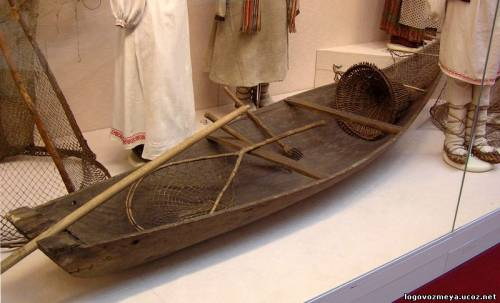
\includegraphics[height=6cm]{dolb_ship.jpg}
      \hfil
      %%\end{minipage}
  %%\end{center}

  %% \begin{itemize}
  %% \item Запрос-ответ
  %% \item Малое время жизни
  %% \item Не следим за ресурсами
  %% \item Не нужна сборка мусора
  %% \item ... и не только она
  %% \end{itemize}
\end{frame}

\begin{frame}
  \frametitle{Стало}
      \hfil
      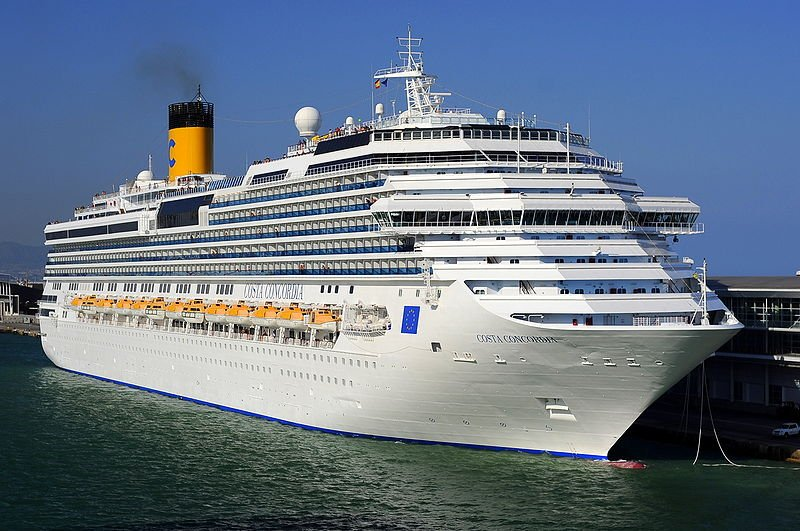
\includegraphics[height=6cm]{costa_concordia.jpg}
      \hfil
  %% \begin{itemize}
  %% \item Много долгоживущих соединений
  %% \item Много ядер CPU
  %% \item Большое время жизни
  %% \item Надо следить за ресурсами
  %% \item Нужна сборка мусора
  %% \item ... и не только она
  %% \end{itemize}
\end{frame}

\begin{frame}
  \frametitle{Что делать?}
  \begin{itemize}
    \pause
  \item \textbf{\color{darkgray}PHP, Ruby, Python etc.}
  \item \textbf{\color{darkgray}Node.js}
  \item \textbf{\color{darkgray}Erlang/OTP}
  \end{itemize}
\end{frame}

\begin{frame}
  \frametitle{SMP — Symmetric Multiprocessing}
  \begin{center}
    \begin{tabular}{| r | l |}
      \hline
      \textbf{\color{darkgray}Обычные языки} & \textbf{\color{red}NO WAY} \\ \hline
      \textbf{\color{darkgray}Node.js} & \textbf{\color{red}Не, не слышал} \\ \hline
      \textbf{\color{darkgray}Erlang} & \textbf{\color{darkgreen}Лучше всех} \\
      \hline
    \end{tabular}
  \end{center}
\end{frame}

\begin{frame}
  \frametitle{CPU}
  \begin{center}
    \begin{tabular}{| r | l |}
      \hline
      \textbf{\color{darkgray}Обычные языки} & \textbf{\color{red}Много} \\ \hline
      \textbf{\color{darkgray}Node.js} & \textbf{\color{darkgreen}Нормально} \\ \hline
      \textbf{\color{darkgray}Erlang} & \textbf{\color{darkgreen}Меньше всех} \\
      \hline
    \end{tabular}
  \end{center}
\end{frame}

\begin{frame}
  \frametitle{Memory}
  \begin{center}
    \begin{tabular}{| r | l |}
      \hline
      \textbf{\color{darkgray}Обычные языки} & \textbf{\color{red}Дохрена} \\ \hline
      \textbf{\color{darkgray}Node.js} & \textbf{\color{darkgreen}Нормально} \\ \hline
      \textbf{\color{darkgray}Erlang} & \textbf{\color{darkgreen}Меньше всех} \\
      \hline
    \end{tabular}
  \end{center}
\end{frame}

\begin{frame}
  \frametitle{Отладка}
  \begin{center}
    \begin{tabular}{| r | l |}
      \hline
      \textbf{\color{darkgray}Обычные языки} & \textbf{\color{blue}Сойдёт} \\ \hline
      \textbf{\color{darkgray}Node.js} & \textbf{\color{red}ОЛОЛО} \\ \hline
      \textbf{\color{darkgray}Erlang} & \textbf{\color{darkgreen}Лучше всех} \\
      \hline
    \end{tabular}
  \end{center}
\end{frame}

\begin{frame}
  \frametitle{Язык}
  \begin{center}
    \begin{tabular}{| r | l |}
      \hline
      \textbf{\color{darkgray}Обычные языки} & \textbf{\color{blue}Привычно} \\ \hline
      \textbf{\color{darkgray}Node.js} & \textbf{\color{red}Знакомо} ({\color{blue}\url{wtfjs.com}}) \\ \hline
      \textbf{\color{darkgray}Erlang} & \textbf{\color{darkgreen}Просто} \\
      \hline
    \end{tabular}
  \end{center}
\end{frame}

\begin{frame}
  \frametitle{Erlang}
  \begin{itemize}
  \item \textbf{\color{darkgray}Нет} \textbf{\color{magenta}shared memory}
  \item \textbf{\color{darkgray}1} \textbf{\color{magenta}соединение} — \textbf{\color{darkgray}1} \textbf{\color{magenta}процесс}
  \item \textbf{\color{darkgray}Fast} \textbf{\color{magenta}GC}
  \item \textbf{\color{darkgray}True Real Hardcore Oldschool} \textbf{\color{magenta}SMP}
  \end{itemize}
\end{frame}


\begin{frame}
  \frametitle{Erlang}
  \begin{itemize}
  \item \textbf{\color{darkgray}Обработки ошибок}
  \item \textbf{\color{darkgray}Кластеризация}
  \item \textbf{\color{darkgray}Горячая замена кода}
  \end{itemize}
\end{frame}


\begin{frame}
  \frametitle{Nitrogen}
  \begin{itemize}
  \item \textbf{\color{darkgray}Поддерживает Mochiweb, Yaws, Webmachine, Inets}
  \item \textbf{\color{darkgray}Event-Driven Development}
  \item \textbf{\color{darkgray}Лёгкие изменения} %% Замена части страницы в одну строчку
  \item \textbf{\color{darkgray}Шаблоны}
  \item \textbf{\color{darkgray}JQuery-friendly}
  \end{itemize}
\end{frame}


\begin{frame}
  \frametitle{Ресурсы}
  \begin{itemize}
  \item {\color{blue}\url{http://nitrogenproject.com}}
  \item {\color{blue}\url{http://erlang-russian.org}}
  \item {\color{blue}\url{http://erlang.org}}
  \item erlang-programming, erlang-russian на гуглогруппах
  \item {\color{blue}\url{http://github.com/Zert/codefest-2012-web-erlang}}
  \end{itemize}
\end{frame}


\begin{frame}
  \frametitle{Вопросы?}
  \titlepage
\end{frame}


\end{document}
